\documentclass[a4paper,12pt]{report}
%general packages
\usepackage[T2A]{fontenc}
\usepackage[utf8]{inputenc}
\usepackage[english,russian]{babel}
\usepackage{circuitikz}
\usepackage{wrapfig}
\usepackage{makecell}
\usepackage{tabularx}
\usepackage{graphicx}
\usepackage{gensymb}
\usepackage{cancel} %cancel symbol
\usepackage{amsmath,amsfonts,amssymb,amsthm,mathtools}
\usepackage[dvipsnames]{xcolor}

%fancy header + geometry
\usepackage{fancyhdr}
\usepackage[a4paper,includehead,nomarginpar,left=15mm,right=15mm,top=15mm,headheight=10mm,bottom=20mm]{geometry}

%pgfplots
\usepackage{pgfplots}
\usepackage{pgfkeys}
\pgfplotsset{compat=1.12}
\usepackage{mathrsfs}

%multi column text
\usepackage{blindtext}
\usepackage{multicol}

%tikz (draw)
\usepackage{tikz}
\usepackage{pstricks-add}
\usetikzlibrary{intersections}
\usetikzlibrary{arrows.meta}
\usetikzlibrary{calc,angles,positioning}
\usetikzlibrary{arrows}
\usepackage{float}
\usepackage{filecontents}

%parskip settings
\parindent=0ex
\setlength{\parskip}{\baselineskip}%
\setlength{\parindent}{0pt}%

%fancy notation for sets
\newcommand{\R}{{\mathbb R}}
\newcommand{\N}{{\mathbb N}}
\newcommand{\fancy}[1]{{\mathbb{#1}}}
%sgn function
\DeclareMathOperator{\sgn}{sgn}

% intersection and union symbols
\newcommand{\uni}{\cup}
\newcommand{\inter}{\cap}
\newcommand{\re}{\text{Re}}
\newcommand{\const}{\text{const}}

\renewcommand{\footrulewidth}{0.4pt}

%\newcommand{\celsius}{$\ ^\circ C$}

%environments

\newtheorem{problem}{Задача}[]
\newenvironment{sol}{\paragraph{Решение}}{}
\renewcommand\thesection{\arabic{section}}

\usepackage{titlesec}
\titlespacing*{\section}
{0cm}{\baselineskip}{0pt}
\titlespacing*{\subsection}
{0pt}{0.1\baselineskip}{0.1\baselineskip}
\titlespacing*{\paragraph}
{0pt}{0.1\baselineskip}{\baselineskip}

\setcounter{secnumdepth}{0}

\begin{document}
	

\begin{titlepage}
	\begin{center}
		МОСКОВСКИЙ ФИЗИКО-ТЕХНИЧЕСКИЙ ИНСТИТУТ (НАЦИОНАЛЬНЫЙ ИССЛЕДОВАТЕЛЬСКИЙ УНИВЕРСИТЕТ) \\
		
		
		\hfill \break
		Факультет обшей и прикладной физики\\
		\vspace{2.5cm}
		\large{\textbf{Отчёт по лабораторной работе 1.2.5 <<Исследование прецессии уравновешенного гороскопа>>}}\\
		\hfill \break
		\\
	\end{center}
	
	\begin{flushright}
		Выполнил:\\
		Студент гр. Б02-304\\
		Головинов. Г.А.
	\end{flushright}
	
	\vspace{7cm}
	
	\begin{center}
		
\includegraphics[width=0.15\linewidth]{uni}
	\end{center}
	

	

	\vfill
	
	\begin{center} Долгопрудный, 2023 \end{center}
	
	\thispagestyle{empty}
	
\end{titlepage}


	\newpage
	%\pagenumbering{arabic}
    \pagestyle{fancy}

    \fancyhead{}
    \fancyfoot{}
    \fancyhead[L]{\rightmark}
    \fancyhead[R]{\thepage}
    \fancyfoot[R]{Работа 2.2.1. --- Взаимная диффузия}

    \section*{Аннотация}
        \paragraph*{Цель работы:} получить зависимость коэффициента диффузии от давления
        \paragraph*{В работе используются:} компьютерезированная установка для измерений, манометр, барометр (для определения атмосферного давления). 
    \vspace{0.5cm}
    \hrule

    \section{Основные теоретические сведения}
    \begin{multicols}{2}
        \emph{Диффузия} --- самопроизвольное взаимное проникновение веществ друг в друга, происходящее вследствие теплового движения молекул.

        Диффузия двух веществ подчиняется закону Фика: плотности потока компонентов $j_{a,b}$ --- количество частиц, пересекающих единичную площадку в единицу времени --- пропорциональны градиентам концентраций $\nabla n_{a,b}$. В одномерном случае:
        \begin{equation*}
            j_a=-D\frac{\partial n_a}{\partial x}, \quad j_b=-D\frac{\partial n_b}{\partial x},
        \end{equation*}
        где $D$ --- коэффициент взаимной диффузии.

        В нашем опыте исследуется взаимная диффузия гелия и воздуха. Причем мы считаем, что давление и температура в процессе опыта не изменяется, поэтому для любых изменений справедливо $\Delta n_1=-\Delta n_2$, где индексом <<1>> будем обозначать воздух, <<2>> --- гелий. Тогда достаточно описать диффузию одного компонента, например воздуха:
        \begin{equation}
            j_1=-D\frac{\partial n_1}{\partial x}
        \end{equation}
        В работе мы используем малые концентрации гелия, поэтому можно приблизить $n_2 \ll n_1$. Кроме того, гелий намного меньше воздуха ($\mu_\text{He}\ll \mu_{\text{N}_2},\mu_{\text{O}_2}$), поэтому скорость частиц гелия много больше скорости частиц воздуха, поэтому его можно вообще считать стационарным. В таком случае коэффициента диффузии равен:
        \begin{equation}
            D=\frac{1}{3}\lambda \bar{v}
        \end{equation}
        где $\bar{v}=\sqrt{\frac{8RT}{\pi\mu}}$ --- средняя тепловая скорость частиц, $\lambda=\frac{1}{n\sigma}$ --- длина свободного пробега, $n$ --- концентрация фона, $\sigma$ --- сечение столкновения примеси с фоном.

        Таким образом, $D\sim\lambda\sim\frac{1}{n}\sim\frac{1}{p}$.
    \end{multicols}

    \hrule
    \begin{multicols}{2}
    \begin{figure}[H]
        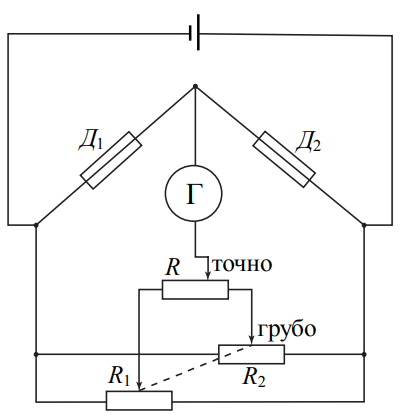
\includegraphics[width=0.64\columnwidth]{../img/schematic.png}
        \centering
        \caption{Схема моста}
        \label{fig:1}
    \end{figure}
    \newcolumn
    \begin{figure}[H]
        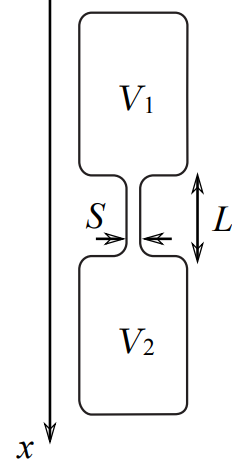
\includegraphics[width=0.35\linewidth]{../img/volumes.png}
        \centering
        \caption{Расположение сосудов с веществами}
        \label{fig:2}
    \end{figure}
    \end{multicols}

    \newpage
    \section{Схема эксперимента}
    \begin{multicols}{2}
        Если на концах трубки, соединяющей сосуды, поддерживается постоянная концентрация гелия (это можно принять так, выходит из предыдущих приближений), то распределение концентрации в трубке $n(x)$ --- линейная функция:
        \begin{equation}
            n(x)=\frac{\Delta n}{L}x
        \end{equation}
        где $L$ --- длина трубки, $\Delta n = n_2-n_1$ --- разница концентраций гелия на концах трубки.

        Плотность потока частиц всюду постоянная и равна:
        \begin{equation}
            j=-D\frac{\Delta n}{L}
        \end{equation}

        Концентрации на концах $n_1,n_2$ меняются со временем (так как гелий переходит из одного сосуда в другой). Предположим, что изменение мало и за это время успевает установиться стационарное течение. $N_1=n_1V$, $N_2=n_2V$ --- полное число частиц. Через него можно выразить поток:
        \begin{equation}
            \frac{dN_1}{dt}=jS, \quad \frac{dN_2}{dt}=-jS
        \end{equation}
        Тогда можно выразить скорость изменения $\Delta n$:
        \begin{equation}
            \frac{d(\Delta n)}{dt}=-\frac{\Delta n}{\tau}, \quad \tau=\frac{1}{D}\cdot\frac{VL}{2S}
        \end{equation}
        Интегрируя, получим $\Delta n = \Delta n_0 \exp{(-t/\tau)}$
        Отсюда видно, что $\tau$ --- характерное время выравнивания концентраций между сосудами.
    \end{multicols}
    \vspace{1cm}
    \hrule
    \section{Методика измерений}
    \begin{multicols}{2}
        Для измерения разности концентраций применяются датчики теплопроводности. Теплопроводность $\varkappa$ зависит от концентрации при малых ее изменениях следующим образом:
        \begin{equation}
            \Delta\varkappa=\varkappa(n_2)-\varkappa(n_1)\approx\text{const}\cdot\Delta n
        \end{equation}
        Для разных концентраций гелия соответственно разная теплопроводность смеси, соответственно разная температура нити (если теплопроводность хуже, значит температура повысится). Повышение (понижение) температуры нити можно измерить с помощью мостовой схемы, показанной на рисунке \ref{fig:1}.

        При незначительных отличиях в составах смесей показания вольтметра, присоединенного по диагонали в мост будут пропорциональны разнице теплопроводности, которая пропорциональна разнице концентраций:
        \begin{gather*}
            U\sim\Delta\varkappa\sim\Delta n
        \end{gather*}
        Тогда получим зависимость показания вольтметра от времени:
        \begin{equation}
            U(t)=U_0\exp{(-t/\tau)}
        \end{equation}
        где $U_0$ --- начальное показание вольтметра.
    \end{multicols}
    \hrule 
    \newpage

    \begin{figure}[H]
    \centering
    \begin{tikzpicture}
        \begin{axis}[
            title={Measured transfer function of analogue filter},
            grid=both,
            minor grid style={gray!25},
            major grid style={gray!25},
            width=0.75\linewidth,
            no marks,
            xlabel={$t$, сек.},
            ylabel={$U$, мВ}
            ]
        \addplot[line width=1pt,solid,color=blue] %
            table[x=T,y=U,col sep=comma]{../data/20240326_1711439001210_41.csv};
        \addlegendentry{$p=41 \ \text{торр}$};
        \addplot[line width=1pt,solid,color=red] %
            table[x=T,y=U,col sep=comma]{../data/20240326_1711440200344_48.5.csv};
        \addlegendentry{$p=48.5 \ \text{торр}$};
        \addplot[line width=1pt,solid,color=black] %
            table[x=T,y=U,col sep=comma]{../data/20240326_1711441128597_59.5.csv};
        \addlegendentry{$p=59.5 \ \text{торр}$};
        \addplot[line width=1pt,solid,color=blue,dashed] %
            table[x=T,y=U,col sep=comma]{../data/20240326_1711442143126_82.csv};
        \addlegendentry{$p=82 \ \text{торр}$};
        \addplot[line width=1pt,solid,color=red,dashed] %
            table[x=T,y=U,col sep=comma]{../data/20240326_1711443254657_119.csv};
        \addlegendentry{$p=119 \ \text{торр}$};
        \addplot[line width=1pt,solid,color=black,dashed] %
            table[x=T,y=U,col sep=comma]{../data/20240326_1711444306232_201.csv};
        \addlegendentry{$p=201 \ \text{торр}$};
        \addplot[green,dashed,domain=0:600] {24.308*e^(-x/370.53)};

        \end{axis}
        
    \end{tikzpicture}
    \end{figure}
\end{document}
